\documentclass[12pt]{exam}
%\documentclass[12pt]{article}
\usepackage[letterpaper, margin=0.75in]{geometry}
\usepackage{graphicx}
\usepackage{enumitem}
\usepackage{booktabs}
\usepackage{amsmath}
\usepackage{tabularx}
\usepackage{color}

\begin{document}
\footer{}{Page \thepage\ of \numpages}{}

\begin{flushright}
\makebox[0.5\textwidth]{\large Name:\enspace\hrulefill}
\vspace{0.2in}

\makebox[0.5\textwidth]{\large Date:\enspace\hrulefill}
\end{flushright}

\begin{center}

\includegraphics[width=10cm]{../images/logo.png}
\end{center}

\begin{center}
\noindent{\LARGE Conceptual Physics \\ Class 11 Questions \\ April 20th, 2018 \\}
\end{center}

\clearpage

\begin{questions}
\question When you travel east in an airplane, do you gain or lose time relative to someone stationary on the ground? What about when you fly west? Does the same thing happen when you drive east or west in a car? If so, why don't you notice it?
\vspace{0.75in}
\question You throw a ball at 20 m/s at a window 10 m away; 0.5 s later, the ball hits and breaks the window. Could there be a frame of reference in which the window broke before you threw the ball?
\vspace{0.75in}
\question On the surface of the Earth, you set off a flash of light and observe a flash of light 1.4 s later on the Moon; since the Moon is 1.3 light-seconds away, you determine that the second flash happened 0.1 s after the first in your frame of reference. Could there be a frame of reference in which the flash on the Moon happened before the flash on Earth?
\vspace{0.75in}

\question Explain what's wrong with the following statement: When you travel close to the speed of light, your time slows down.
\vspace{0.75in}

\question In 1977, NASA launched the Voyager probes. In 2012, Voyager~1 officially left the solar system and entered interstellar space. It is possible to communicate with the probe via radio signals. If we observe Voyager 1 as travelling away from us at velocity \textit{v}, and if \textit{c} is the speed of light, how fast do we measure the signal pulses to be travelling?
	
	\noindent\begin{center}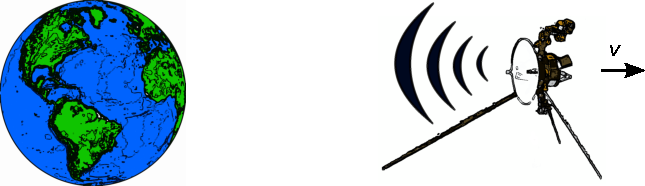
\includegraphics{../images/spacesignal.pdf}\end{center}
	
	\begin{choices}
		\choice $c - v$
		\choice $c$
		\choice $c + v$
		\choice None of the above; radio signals travel instantaneously.
	\end{choices}
	
\clearpage
\question A person in a spaceship moving at 99.99999999\% of the speed
of light relative to Earth shines a flashlight forward through dusty air, so
the beam is visible. What does she see? What would it look like to an
observer on Earth?

From \textit{Light and Matter} Chapter 23, Discussion Question A
\vspace{1in}
	
\question In the following two questions, Abbey is in a spaceship moving at high speed relative to Brendan, who is standing
on an asteroid (a very small piece of rock floating in space). She flies past him so that at t = 0, she is momentarily
adjacent to Brendan.
\noindent\begin{center}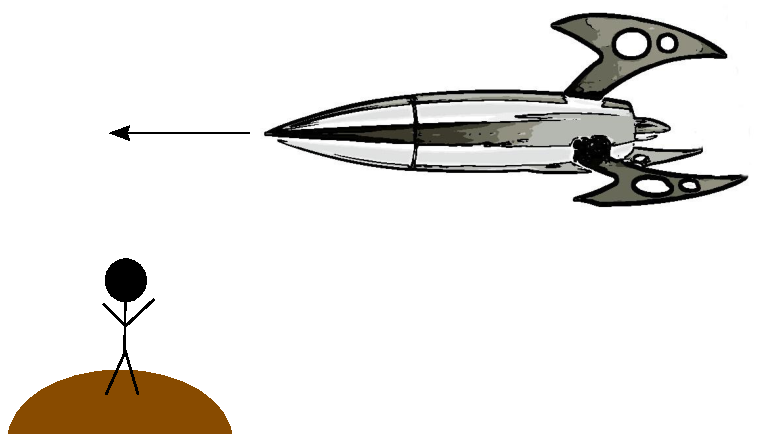
\includegraphics[width=2in]{../images/abbyBrendan.pdf}\end{center}

\begin{parts}
\part At the instant that Abbey’s ship passes Brendan, she sends two light pulses to him from her ship. If the light
pulses are emitted a nanosecond ($10^{-9}$ seconds) apart according to Abbey’s clock, what will be the time interval
between the pulses according to Brendan?
	\begin{choices}
		\choice Greater than one nanosecond
		\choice Equal to one nanosecond
		\choice Less than one nanosecond
	\end{choices}
	
\part Also while Abbey’s ship passes Brendan, Brendan sends two light pulses to Abbey. If Brendan sends the light
pulses a nanosecond ($10^{-9}$ seconds) apart according to his clock, what will be the time interval between the
pulses according to Abbey?
	\begin{choices}
		\choice Greater than one nanosecond
		\choice Equal to one nanosecond
		\choice Less than one nanosecond
	\end{choices}
\vspace{0.3in}
\end{parts}

\question It is known that our galaxy is of the order of 100, 000 light-years in diameter. Is it possible, if travelling at a
constant speed that is less than, but close to, the speed of light, for a person to cross
the galaxy within their lifetime?
\vspace{1in}

\clearpage
\question The Olympic Games is a two-week long sports competition. An interested alien astronomer watches the Olympics
from a distant planet moving at high speed relative to Earth. If the alien were to compensate for the time the
light from Earth takes to reach them, they would measure the length of the Olympics to be:
\begin{choices}
	\choice Greater than two weeks
	\choice Equal to two weeks
	\choice Less than two weeks
\end{choices}

\question Bellow is an artist’s rendering of the length contraction for
the collision of two gold nuclei at relativistic speeds in the RHIC
accelerator in Long Island, New York, which went on line in 2000.
The gold nuclei would appear nearly spherical (or just slightly
lengthened like an American football) in frames moving along with
them, but in the laboratory’s frame, they both appear drastically
foreshortened as they approach the point of collision. The later
pictures show the nuclei merging to form a hot soup, in which
experimenters hope to observe a new form of matter.

\begin{center}
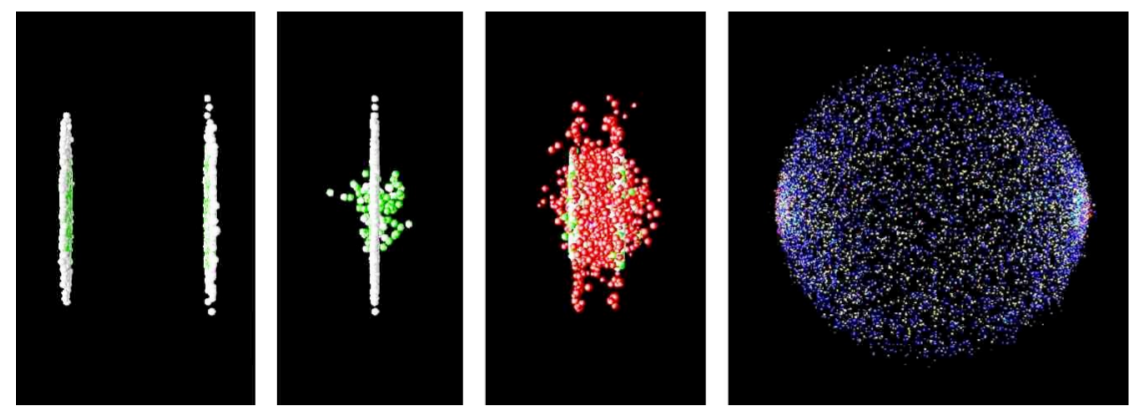
\includegraphics[width=4in]{../images/nuclei.png}
\end{center}

What would the shapes of the two
nuclei look like to a microscopic observer riding on the left-hand nucleus?
To an observer riding on the right-hand one? Can they agree on what is
happening? If not, why not — after all, shouldn’t they see the same thing
if they both compare the two nuclei side-by-side at the same instant in
time?

From \textit{Light and Matter} Chapter 23,  Discussion Question E

\clearpage
\question In the following four questions, Amanda is standing on a train travelling at high speed past Bryan, who is standing
on a platform. As she passes Bryan, she drops two bowling balls out of the window at the same time (Amanda’s
time), and from an arm’s span apart.
\begin{center}
\input{../images/bowlingTrains.pdf_tex}
\end{center}
\begin{parts}
\part Bryan stands on the platform and watches the balls fall to the ground. If he compensates for the time that the
light from the impacts takes to reach him, in what order does Bryan measure the balls hitting the ground?
	\vspace{0.75in}

\part Charlotte is another passenger on the train with Amanda. If she compensates for the time that the light from
the impacts takes to reach her, in what order does Charlotte measure the balls hitting the ground?
	\vspace{0.75in}

\part Amanda has an arm span of D meters at rest. If Bryan performs a measurement of Amanda's arm span as she
passes him, he will obtain a value:
\begin{choices}
	\choice Greater than D
	\choice Equal to D
	\choice Less than D
\end{choices}

\part Amanda also has a height of H meters at rest. If Bryan performs a measurement of Amanda's height as she
passes him, he will obtain a value:
\begin{choices}
	\choice Greater than H
	\choice Equal to H
	\choice Less than H
\end{choices}
\end{parts}

\clearpage 
\question In the following thought experiment, you are in a high speed train travelling along a railway. If
you measure the rate at which your watch is ticking, will you obtain a different value than if the train were at
rest?
\vspace{0.5in}

\question You are still in a high speed train travelling along a railway. If
you measure the dimensions of the train compartment, will you obtain different values than if the train were at
rest?
\vspace{0.5in}


\question You are in a well equipped physics lab without windows or ways of interacting with the outside world. It is
known that the lab is in uniform motion. How do you determine the velocity of the lab?
\begin{choices}
	\choice You throw a ball across the lab and measure its change in velocity
	\choice You shine a laser beam across the lab and measure its change in velocity
	\choice Either (a) or (b)
	\choice It is not possible to determine the lab’s velocity by experiment
\end{choices}
\question Muons are a fundamental particle, similar to the electron but with a much larger mass. A muon will decay about $2.2~\mu\text{s}$ after it is created, into an electron, a neutrino (another fundamental particle) and an ``anti-neutrino" (another fundamental particle).
\begin{eqnarray}
\mu^- \rightarrow e^- + \nu + \bar{\nu} \nonumber
\end{eqnarray}
Physicists study muons, by accelerating them to relativistic speeds in laboratories. The time it takes to decay is called the lifetime of a particle.
	\begin{parts}
		\part From the perspective of a scientist in the lab, will the lifetime of a muon be:
		\begin{choices}
			\choice longer than $2.2~\mu\text{s}$
			\choice shorter than $2.2~\mu\text{s}$
			\choice exactly $2.2~\mu\text{s}$
		\end{choices}
		\part Muons travel from one side of the lab to the other. If physicists measure the length of a lab to be 20~m, then from the perspective of the muon the lab is:
		\begin{choices}
			\choice longer than 20~m
			\choice shorter than 20~m
			\choice exactly 20~m
		\end{choices}
	\end{parts}

\end{questions}


\end{document}
